\documentclass[conference]{IEEEtran}
\IEEEoverridecommandlockouts
\usepackage{cite}
\usepackage{fontspec}
\setmainfont{TeXGyreTermesX}
\usepackage{amsmath,amssymb,booktabs,array}
\usepackage{graphicx}
\usepackage{url}
\usepackage{tikz}
\usetikzlibrary{positioning,arrows.meta}
\usepackage{algorithm}
\usepackage{algpseudocode}
\usepackage{balance}

\title{MIRAGE-OT: Evidence-Grounded Incident Reconstruction and Provenance-Constrained Scenario Synthesis for Operational Technology Networks}

\author{\IEEEauthorblockN{PoTing Lu}
\IEEEauthorblockA{\textit{AvocadoAI Co., Ltd.}\\
Taipei, Taiwan}
\and
\IEEEauthorblockN{Eric Mao\thanks{Corresponding author: Eric Mao.}}
\IEEEauthorblockA{\textit{AvocadoAI Co., Ltd.}\\
Taipei, Taiwan\\
eric.mao@mail.avocadolab.ai}
\and
\IEEEauthorblockN{Shih-Hao Chang}
\IEEEauthorblockA{\textit{Department of Computer Science and Information Engineering}\\
\textit{National Taipei University of Technology}\\
Taipei, Taiwan\\
sh.chang@ntut.edu.tw}}

\begin{document}
\maketitle

\begin{abstract}
Process-aware intrusion detectors can flag a suspicious operational-technology (OT) window, but an alert does not say what happened, which records support it, or what the capture cannot decide.
Answering those questions from packet captures is error-prone: mirror ports duplicate frames, one IEC~60870-5-104 ASDU carries many objects, and state transcriptions re-encode the same messages, so naive correlation multiplies weak evidence.
MIRAGE-OT is a deterministic post-alert method that runs downstream of a detector.
It reconstructs control transactions and sustained measurement steps, admits a relation only when protocol, quality, persistence, and direction evidence agree, and otherwise abstains.
A four-layer synthesis counts each ASDU as one source, bridges two RTUs only on the same grid element, and lists competing explanations together with the evidence that would separate them.
On all 103 Sherlock~v3 test windows, with parameters fixed after the first scenario, every window completes and 102/103 pass full lineage consistency.
A time-proximity-only baseline emits 107{,}666 candidate links inside 15\,s, of which 66{,}706 violate an explicit evidence constraint.
An offline comparison with simulator snapshots, which never enter the engine, finds all 15 verified command transitions and 138 of 142 bridge attributes compatible, with 20 of 23 bridges compatible at every endpoint.
\end{abstract}

\begin{IEEEkeywords}
operational technology, IEC 60870-5-104, incident reconstruction, evidence provenance, abstention
\end{IEEEkeywords}

\section{Introduction}
Detection of attacks on industrial control systems has matured.
Detectors flag departures from learned signal behavior~\cite{aoudi2018pasad}, physical invariants~\cite{feng2019invariants}, compact process features~\cite{wolsing2022simple}, or protocol specifications~\cite{hotellier2024specification}.
Their output is an alert: a time window, a score, and at most an attack-family label.

An alert is where incident response begins, not where it ends.
A responder still has to establish which commands were sent and executed, which grid elements changed state, whether reports from different remote terminal units (RTUs) describe one event, and which questions the capture cannot settle.
Incident-response frameworks for industrial systems describe these steps~\cite{smith2021air4ics,staves2022incidentresponse}, but they leave the evidence work to the analyst.

Doing that work from packet captures has two traps.
The first is evidence inflation.
The same frame is captured at several mirror ports, one application service data unit (ASDU) reports dozens of information objects, and state transcriptions such as IPAL~\cite{wolsing2022ipal} re-encode the same message.
Counted naively, one report becomes many confirmations.
The second is over-association.
In a disturbed grid many measurements change within seconds of one another, and temporal proximity is easily read as causation.
A capture also lacks the bus-branch model and relay records that would decide physical causation, so a single causal graph is not identifiable from packets alone.

These gaps motivate a separate, downstream task: explaining a window that a detector has already flagged.
MIRAGE-OT takes such a window and returns an evidence-bounded scenario.
Relations are supported where the protocol and the samples agree, unresolved where they do not, and every competing explanation names the evidence that would decide it.
MIRAGE-OT neither detects nor classifies attacks.
It reads switch captures and IPAL state, and it does not read event labels, attack names, or simulator state.
The contributions are as follows.
\begin{itemize}
\item \textbf{C1, protocol-aware and behavioral reconstruction.} IEC~60870-5-104 control transactions~\cite{iec60870} and sustained measurement or state steps are reconstructed, so that windows without any control command still yield structure.
\item \textbf{C2, evidence-constrained verification with abstention.} A relation is supported only when stated telemetry constraints hold; otherwise it stays unresolved or is quarantined.
\item \textbf{C3, provenance-constrained synthesis.} One ASDU counts as one source, cross-RTU bridges require the same grid element, and competing explanations carry their missing evidence. A bridge records an observed two-end transition, not a physical cause.
\end{itemize}
Table~\ref{tab:claims} maps each contribution to the comparison that tests it on all 103 Sherlock~v3 test windows~\cite{wagner2025sherlock,sherlockv3}.

\begin{figure*}[t]
\centering
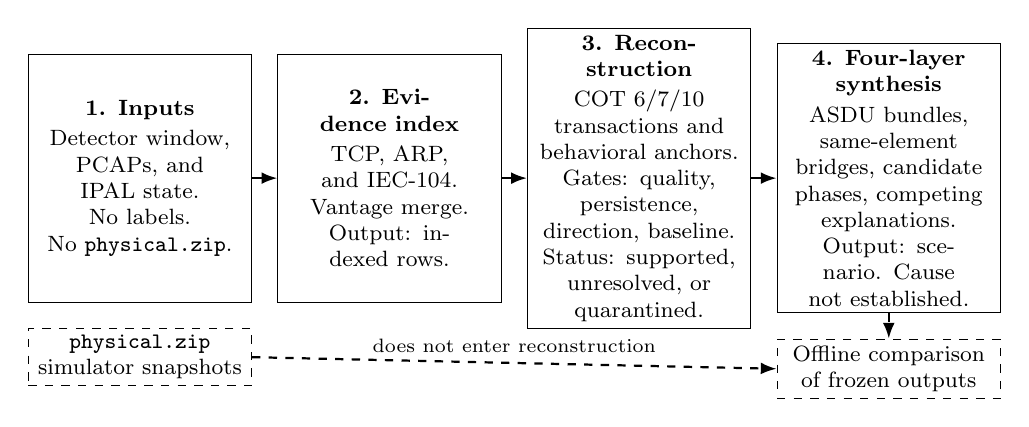
\begin{tikzpicture}[
  font=\footnotesize,
  node distance=3.2mm,
  stage/.style={draw, align=center, inner sep=2.4pt, text width=0.22\textwidth, minimum height=3.15cm},
  side/.style={draw, dashed, align=center, inner sep=2.4pt, text width=0.22\textwidth},
  arr/.style={-{Latex[length=2mm]}, thick},
  darr/.style={-{Latex[length=2mm]}, thick, dashed}
]
\node[stage] (in) {\textbf{1. Inputs}\\[1.5pt]
Detector window, PCAPs, and IPAL state.\\
No labels.\\
No \texttt{physical.zip}.};
\node[stage, right=of in] (idx) {\textbf{2. Evidence index}\\[1.5pt]
TCP, ARP, and IEC-104.\\
Vantage merge.\\
Output: indexed rows.};
\node[stage, right=of idx] (rec) {\textbf{3. Reconstruction}\\[1.5pt]
COT 6/7/10 transactions and behavioral anchors.\\
Gates: quality, persistence, direction, baseline.\\
Status: supported, unresolved, or quarantined.};
\node[stage, right=of rec] (syn) {\textbf{4. Four-layer synthesis}\\[1.5pt]
ASDU bundles, same-element bridges, candidate phases, competing explanations.\\
Output: scenario. Cause not established.};
\node[side, below=of in] (phys) {\texttt{physical.zip}\\
simulator snapshots};
\node[side, below=of syn] (off) {Offline comparison\\
of frozen outputs};
\draw[arr] (in) -- (idx);
\draw[arr] (idx) -- (rec);
\draw[arr] (rec) -- (syn);
\draw[darr] (syn.south) -- (off.north);
\draw[darr] (phys.east) -- node[above, font=\scriptsize] {does not enter reconstruction} (off.west);
\end{tikzpicture}
\caption{Four stages from a detector's window to a scenario. Solid arrows are reconstruction inputs and outputs. The dashed path compares frozen outputs with simulator snapshots and does not enter the engine. A same-element bridge is an observation; its cause remains unresolved.}
\label{fig:arch}
\end{figure*}

\section{Related Work}
The detectors above score anomalies; MIRAGE-OT starts from their output.
Cross-domain correlation combines cyber and physical alerts in industrial control systems~\cite{koucham2022crossdomain}, but it relates alerts rather than the packet records beneath them.
Incident-response frameworks organize operator procedure~\cite{smith2021air4ics,staves2022incidentresponse}.
MIRAGE-OT supplies an input to that procedure: a window graph whose relations keep packet-level evidence references and explicit unresolved states.
The IPAL format provides a common representation of industrial traffic and state for detection research~\cite{wolsing2022ipal}.
Here an IPAL row and a dissected ASDU can be two encodings of one message, and the synthesis gives the IPAL copy zero independent weight.

\section{MIRAGE-OT Methodology}
\subsection{Evidence index and anchors}
A window is an interval $I=[t_s,t_e)$ plus a short background.
The index stores TCP and ARP frames, IEC-104 ASDUs dissected from every capture, and IPAL rows marked as network-reported state.
Copies of one frame at different mirror ports within 0.5\,s are merged; if their payloads disagree, the anchor is marked with a cross-vantage conflict and quarantined.
Each mapped point has an entity name such as \texttt{line.3:current\_from}; its \emph{device stem} is the grid element before the colon (\texttt{line.3}).
Fig.~\ref{fig:arch} shows the path from capture to scenario.

A measurement sample $v_k$ is a step from $v_{k-1}$ when it falls to near zero ($|v_k|<10^{-3}$), rises from near zero, or changes by a relative amount $|v_k-v_{k-1}|/\max(|v_k|,|v_{k-1}|)\ge 0.5$.
The step becomes an anchor only if the previous sample is at most 30\,s old, both samples have good quality and a clear test bit, and the step persists: at least two later samples, at least 80\% of them consistent with the new value (within 10\%, or near zero for a drop to zero).
A state report becomes an anchor when the state differs from an in-window prior value; with no prior value it is kept as an unverified precursor.
Link anchors mark IEC-104 telemetry gaps longer than $\max(25\,\mathrm{s}, 3\times$ the median background cadence$)$, and ARP anchors mark at least 10 ARP packets and at least five times the background rate.
These parameters were set during development on Basic and were not changed afterward.

\subsection{Verification and abstention}
A control transaction is a cause-of-transmission (COT)~6 activation, a COT~7 confirmation with the negative bit clear, and, when present, a COT~10 termination~\cite{iec60870}.
It is a verified transition only when pre-command and post-command samples differ in the direction the command states.
Without an IEC-104 pre-command sample, the status is \texttt{state\_report\_observed\_no\_pre\_baseline}, and the command is kept for audit, not verified.

Two anchors form a corroborated same-element transition only if all of the following hold: the same device stem; separate ASDUs; $0\le\Delta t\le 15$\,s; both anchors verified; transition intervals aligned within 1\,s; and complementary line ends (\texttt{from}/\texttt{to}) sharing a quantity with the same step kind.
For level shifts the magnitudes must move in the same direction with a ratio agreement of at least 0.5, and active power must reverse sign across the two ends.
A state report followed by a flow step must match open-to-zero or close-from-zero.
Same-ASDU co-reports are one container, not a sequence.
Pairs inside 15\,s without this evidence stay unresolved; they are not labeled false.
Pairs that violate quality, persistence, change type, direction, or vantage consistency are explicit conflicts.

\subsection{Provenance-constrained synthesis}
Algorithm~\ref{alg:syn} lists the four layers as implemented.
Layer~1 partitions local storylines.
Layer~2 groups verified anchors by ASDU, so a bundle counts as one independent source however many objects or mirror ports it has.
A bridge joins two bundles only through a supported same-element transition that passes the gate again, and only across distinct RTUs; a same-RTU relation is kept but is not a bridge.
Co-reported neighbors of a bridged element are not connected by it.
Layer~3 forms candidate phases by start time alone.
RTU, master, and ARP-target overlap are recorded as phase context, and all cross-device links inside a phase stay unresolved.
Layer~4 builds a source-dependency ledger and emits competing explanations from fixed rule templates.
The templates fire on what the window contains: command transactions; cross-RTU bridges, which yield a switching or protection-cascade hypothesis and an uncommanded or altered-telemetry hypothesis; link-change anchors, with shared-path and independent-RTU hypotheses, or ARP variants graded by per-target precedence when ARP anchors exist; or, failing all of these, a same-element sequence that failed the gate.
A window that triggers no template receives no explanation.
Explanations are not ranked, and each lists \texttt{missing\_disambiguating\_evidence}, such as a bus-branch model or a relay trip record.

\begin{algorithm}[t]
\caption{Four-layer synthesis for one window}
\label{alg:syn}
\footnotesize
\begin{algorithmic}[1]
\Require transactions $T$, anchors $A$, event graph $G$, storylines $S$
\State \textbf{L1:} split $S$ into supported chains, verified single anchors, same-element sequences that failed the gate, and quarantined anchors; mark state reports with no in-window prior as precursors
\State \textbf{L2:} $B\gets$ verified anchors not covered by $T$, grouped by ASDU; each $b\in B$ has one independent source
\For{each supported same-element edge $(u,v)\in G$ with $u,v$ in bundles of $B$}
  \If{gate$(u,v)$ passes, $b(u)\neq b(v)$, and $\mathrm{rtu}(u)\neq\mathrm{rtu}(v)$}
    \State add bridge $(b(u),b(v))$; claim: observed; cause: not established
  \EndIf
\EndFor
\State \textbf{L3:} sort $T\cup B\cup$ precursors by start time; open a new phase when the gap to the latest start in the current phase exceeds 15\,s; attach bridges and unresolved candidates
\State \textbf{L4:} write the ledger (containers, RTUs, vantages; IPAL weight 0); emit each template explanation whose trigger is present, with its missing evidence
\State \Return bundles, bridges, phases, ledger, explanations
\end{algorithmic}
\end{algorithm}

\section{Experimental Setup}
\textbf{Dataset.}
Sherlock~v3 is a power-grid dataset for process-aware intrusion detection~\cite{wagner2025sherlock,sherlockv3}.
Its three scenarios run a control center and RTUs that speak IEC~60870-5-104 over simulated medium-voltage grids.
The dataset configuration names the CIGRE MV grid for Basic and SimBench MV semi-urban and rural grids for Semiurban and Rural.
Test runs combine a baseline operation playbook with attack playbooks named Industroyer, drift-off, control-and-freeze, and ARP spoofing.
Each scenario provides switch captures from several mirror ports, IPAL state transcriptions, event labels, and \texttt{physical.zip}, a series of simulator snapshots taken every 0.5--2\,s.
We evaluate all 103 test windows: 28 Basic (500 mapped points, 4 mirror vantages), 39 Semiurban (3{,}640 points, 6 vantages), and 36 Rural (1{,}908 points, 8 vantages).
Event labels and \texttt{physical.zip} are excluded from indexing and reconstruction.
The engine and its parameters were frozen after Basic and transferred unchanged to Semiurban and Rural.

\textbf{Comparisons.}
\emph{Time-Proximity-Only} (B1) links the same anchors within the same 15\,s horizon, capping cross-device links at six per anchor and keeping all same-device and same-ASDU pairs.
It sorts candidates into those flagged by an explicit constraint, unsubstantiated candidates, and same-device candidates with no detected conflict; the last is a baseline category, not a MIRAGE-OT supported relation.
\emph{Control-Transaction-Only} (B2) keeps the COT~6/7/10 rules and does not apply to a window with no control object.
Three ablations are computed on the frozen outputs and quantify what one component withholds or adds; they do not rerun a modified engine.
\emph{Gate-rejected promotions} (A1) counts the same-device pairs that the behavioral or command gate rejected.
\emph{Provenance accounting} (A2) attributes raw observation rows to mirror duplicates, extra objects in one ASDU, IPAL rows, and multi-event anchors.
A row is a mirror duplicate only across distinct vantages within 0.5\,s and with the same packet identity (for IEC-104, flow, transmit sequence number, ASDU index, address, and object index); a row lacking those fields is counted as unknown.
\emph{Synthesis-off} (A3) stops at local storylines.

\textbf{Traceability (E3)} has four nested checks per window: \emph{citation presence}, where every emitted bundle and bridge cites evidence and every explanation cites anchoring and missing evidence; \emph{evidence-ID resolution}, where every cited identifier exists in the window's index; \emph{fact and anchor consistency}, where every cited row matches its fact or anchor on entity, CA/IOA, device or host, and time window; and \emph{full lineage consistency}, which adds the engine's own lineage flag.
A check over an empty set passes, so coverage matters.
Bundles are empty in 48 windows, bridges in 97, and explanations in 18; only 6 windows contain all three.
One window cites no identifier, and 45 windows check no behavioral anchor.
Bootstrap intervals are descriptive only, because windows cut from one recording share grid state and are not independent.

\textbf{Offline physical comparison.}
After freezing, the outputs of all three scenarios are compared with their snapshots: 40{,}319 for Basic (0.5--2\,s apart) and about 22{,}000 each for Semiurban and Rural (mostly 2\,s apart), using the nearest snapshot without interpolation.
With relative difference $\delta=|v_{\mathrm{phys}}-v_{\mathrm{net}}|/\max(1,|v_{\mathrm{net}}|)$, a comparison is exact when the absolute difference is at most $10^{-3}$ or $\delta\le 10^{-4}$, and within tolerance when $\delta\le 0.05$ for transactions or $\le 0.10$ for bridge points.
A simulator \texttt{NaN} paired with a network value within $10^{-3}$ of zero is semantic compatibility for a de-energized island, not numeric equality.
For a \texttt{to\_zero} step the pre-value is also compared numerically.

\section{Results and Discussion}
\subsection{Cross-scenario reconstruction}
Table~\ref{tab:cross} summarizes the frozen run.
Every window completes.
Citation presence and evidence-ID resolution pass in all 103 windows, and fact/anchor and full lineage consistency in 102/103.
In the exception, Semiurban window \texttt{ev\_5dd0102}, a cross-switch timestamp inconsistency downgrades the report to diagnostic-only.
The consistency check therefore withholds a report rather than passing it.
Semiurban has 15 windows with reconstructed COT~6 transactions and 16 in which B2 applies; the extra window, \texttt{ev\_5dd0102}, contains 62 unpaired COT~7 replies and no matching COT~6 command.
Median reconstruction-and-synthesis time is 0.66\,s on Basic, 14.04\,s on Semiurban, and 7.74\,s on Rural (6.40\,s over all windows), excluding shared indexing.

\begin{table}[t]
\caption{Frozen reconstruction across 103 Sherlock~v3 test windows.}
\label{tab:cross}
\centering
\scriptsize
\setlength{\tabcolsep}{2.2pt}
\begin{tabular}{@{}lrrrr@{}}
\toprule
 & Basic & Semi. & Rural & All \\
\midrule
Windows & 28 & 39 & 36 & 103 \\
B2 applicable / not & 16/12 & 16/23 & 14/22 & 46/57 \\
Verified command transitions & 9 & 3 & 3 & 15 \\
ASDU bundles & 36 & 910 & 754 & 1{,}700 \\
Cross-RTU bridges & 6 & 6 & 11 & 23 \\
Bridged components & 3 & 2 & 6 & 11 \\
Candidate phases & 27 & 55 & 61 & 143 \\
Competing explanations & 46 & 63 & 52 & 161 \\
Storylines if synthesis stops & 1{,}270 & 5{,}518 & 4{,}262 & 11{,}050 \\
E3 citation presence & 28/28 & 39/39 & 36/36 & 103/103 \\
E3 evidence-ID resolution & 28/28 & 39/39 & 36/36 & 103/103 \\
E3 fact/anchor consistency & 28/28 & 38/39 & 36/36 & 102/103 \\
E3 full lineage consistency & 28/28 & 38/39 & 36/36 & 102/103 \\
Recon.\ median / mean (s) & 0.66/0.91 & 14.0/21.2 & 7.74/11.6 & 6.40/12.3 \\
\bottomrule
\end{tabular}
\end{table}

\begin{table}[t]
\caption{Contributions, the comparisons that test them, and what remains unshown (103 windows unless stated).}
\label{tab:claims}
\centering
\scriptsize
\setlength{\tabcolsep}{2.2pt}
\begin{tabular}{@{}>{\raggedright\arraybackslash}p{0.09\columnwidth}>{\raggedright\arraybackslash}p{0.6\columnwidth}>{\raggedright\arraybackslash}p{0.27\columnwidth}@{}}
\toprule
Claim & Comparison and result & Not shown \\
\midrule
C1 & Control-Transaction-Only: applies in 46/103 windows with the same 15 verified transitions; omits 2{,}776 non-command anchors, 23 bridges, and 134 link or ARP anomalies. & Whether omitted anchors aid a responder. \\
C2 & Time-Proximity-Only: 107{,}666 candidates; 66{,}706 constraint-flagged, including 2{,}628 same-ASDU ordering conflicts; 18{,}130 unsubstantiated; 22{,}830 same-device with no detected conflict. Gate-rejected promotions: 2{,}171 (409 bridges); without \texttt{ev\_52f5ee}, 205 (49) in 51/102 windows. & Whether any rejected pair is a true relation. \\
C3 & Provenance accounting: 9{,}836 rows over 4{,}493 containers, excess fully attributed. Synthesis-off: 11{,}050 storylines without bundles, bridges, phases, or explanations. Case study in Sec.~\ref{sec:case}. & Analyst time or comprehension. \\
C1--C3 & Offline simulator check across all scenarios: 15/15 transitions and 138/142 bridge attributes compatible (74 numeric, 64 semantic \texttt{NaN}); 20/23 bridges fully compatible. & Physical causality. \\
\bottomrule
\end{tabular}
\end{table}

\subsection{What each component changes}
Table~\ref{tab:claims} pairs each claim with its test.
For C1, B2 verifies the same 15 command transitions but applies in only 46/103 windows.
On the other 57 it yields no incident structure, whereas the behavioral anchors still reconstruct steps, bridges, and link or ARP anomalies.

For C2, B1 shows how far time proximity alone over-associates.
Its 107{,}666 candidates are 78{,}238 cross-device pairs, 26{,}800 same-device pairs in separate ASDUs, and 2{,}628 same-ASDU co-reports.
Of these, 66{,}706 are flagged by explicit constraints, 18{,}130 are unsubstantiated, and 22{,}830 are same-device candidates with no detected conflict.
The 2{,}628 same-ASDU cases lie inside the 66{,}706; they are ordering conflicts created by treating co-reported objects as a sequence, not measurement contradictions.
Other constraint tags, led by a step that is not sustained (66{,}042 links), cover quality, persistence, direction, and vantage disagreement, and they overlap.
MIRAGE-OT keeps the unsubstantiated set unresolved instead of promoting it.
Descriptive 95\% intervals for the per-window B1-minus-MIRAGE counts are $[435, 882]$ for conflicts and $[126, 237]$ for unsubstantiated candidates.
A1 measures what the gate withholds: 2{,}171 relations in 52/103 windows, including 409 cross-RTU bridges.
One window, \texttt{ev\_52f5ee}, accounts for 1{,}966 of them; without it the gate still withholds 205 relations and 49 bridges in 51/102 windows.
These are rejected pairs, not confirmed false positives.

For C3, A2 explains 5{,}343 excess rows: 1{,}845 mirror duplicates, 572 extra objects in the same ASDU, 2{,}262 IPAL rows, 268 further messages in the same TCP session, and 396 distinct-time events inside one anchor, with no unknown remainder.
The mean per-window inflation factor is 2.44.
A3 leaves 11{,}050 local storylines in place of 1{,}700 bundles, 23 bridges, 143 phases, and 161 explanations.
The case below shows what that organization adds in one window.

\subsection{Case study: a multi-RTU de-energization}
\label{sec:case}
Basic window \texttt{ev\_564bebaa} (180.2\,s) has no control command, so B2 does not apply.
Its 109 raw observation rows reduce to 12 ASDU containers after removing 3 mirror duplicates, 41 extra objects in shared ASDUs, and 53 IPAL rows.
Of 32 anchors, 23 are verified and 9 are quarantined.
B1 emits 157 candidate links: 29 constraint-flagged, 123 unsubstantiated, and 5 same-device candidates with no detected conflict.
The gate supports five same-element transitions, all across distinct RTUs, and withholds three more cross-RTU promotions that A1 counts.

Fig.~\ref{fig:bridge} shows the resulting bridges.
The de-energized component links \texttt{line.3} (RTU 172.16.3.18 at $+5.645$\,s to 172.16.3.16 at $+10.695$\,s), \texttt{line.4} (.18 to .22 at $+7.772$\,s), and \texttt{line.12} (.22 to .24 at $+7.844$\,s), with corroborated \texttt{to\_zero} steps on both ends.
A second component links \texttt{line.0} and \texttt{line.1} as level shifts.
The \texttt{line.3} bridge records both ends reported in separate ASDUs, and it does not connect the co-reported bus, load, and neighboring line.
Layer~3 places all 12 bundles in one phase that holds 129 unresolved cross-device candidates, the same pairs as B1's cross-device candidates, which include its 123 unsubstantiated ones; B1's other 28 pairs are same-ASDU or same-device.
Layer~4 emits two explanations.
A switching or protection cascade lists three missing items: a bus-branch topology, a pre-window baseline for two spontaneous state reports, and relay trip records.
Uncommanded or altered telemetry lists two: out-of-band electrical measurements and RTU logs.
Instead of 157 temporal links, the responder sees five observed bridges in two components, two open hypotheses, and the five missing items that would separate them.

\begin{figure}[t]
\centering
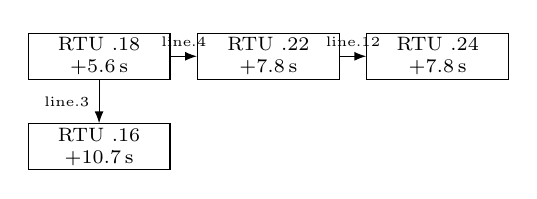
\begin{tikzpicture}[
  font=\scriptsize,
  rtu/.style={draw, align=center, inner sep=1.5pt, minimum width=18mm},
  arr/.style={-{Latex[length=1.5mm]}}
]
\node[rtu] (a) at (0,0) {RTU .18\\$+5.6$\,s};
\node[rtu] (b) at (2.15,0) {RTU .22\\$+7.8$\,s};
\node[rtu] (c) at (4.3,0) {RTU .24\\$+7.8$\,s};
\node[rtu] (d) at (0,-1.15) {RTU .16\\$+10.7$\,s};
\draw[arr] (a) -- node[above, font=\tiny] {line.4} (b);
\draw[arr] (b) -- node[above, font=\tiny] {line.12} (c);
\draw[arr] (a) -- node[left, font=\tiny] {line.3} (d);
\end{tikzpicture}
\caption{Same-element observation bridges in \texttt{ev\_564bebaa}. Arrows are corroborated two-end reports, and causal status is not established. \texttt{line.0} and \texttt{line.1} form a separate level-shift component and are omitted for space.}
\label{fig:bridge}
\end{figure}

\subsection{Physical compatibility and fail-closed cases}
Table~\ref{tab:phys} gives the offline comparison for all three scenarios.
All 15 verified command transitions are numerically compatible: 14 exact and 1 within 5\% (\texttt{sgen.6} active power in Basic \texttt{ev\_0961f1c2}).
Of 142 bridge attributes, 138 are compatible, but only 74 of these are numeric matches (44 exact, 30 within 10\%); the other 64 are semantic \texttt{NaN} on a de-energized island, not numeric equality.
Maximum $|\Delta t|$ is 1.443\,s for transactions (Semiurban) and 1.068\,s for bridge attributes (Rural), reflecting the roughly 2\,s snapshot spacing there.

All four failures are pre-event currents of \texttt{to\_zero} steps, whose \texttt{NaN} post-values do not repair the pre-current mismatch.
Three are in Basic \texttt{ev\_564bebaa}: \texttt{line.4:current\_from} has $\delta=0.153$ (4.713 versus 3.993), \texttt{line.12:current\_from} has $\delta=0.266$ (0.175 versus $-0.092$), and \texttt{line.12:current\_to} has $\delta=0.427$ (0.294 versus $-0.133$).
The fourth is \texttt{line.100:current\_to} in Rural \texttt{ev\_0d966f9}, with $\delta=0.241$ (0.0814 versus $-0.1594$).
Bridges compatible at every endpoint are therefore 20/23: 4/6 in Basic, 6/6 in Semiurban, and 10/11 in Rural.
Four of the six Semiurban bridges are in \texttt{ev\_d3c4667}, where one \texttt{line.6} report from one RTU bridges to four \texttt{line.6} reports from another; with a \texttt{line.7} bridge they form one of Semiurban's two bridged components, so 6/6 does not mean six independent elements.

\begin{table}[t]
\caption{Offline physical comparison of frozen outputs. Semantic \texttt{NaN} is not a numeric match.}
\label{tab:phys}
\centering
\scriptsize
\setlength{\tabcolsep}{3pt}
\begin{tabular}{@{}lrrrr@{}}
\toprule
 & Basic & Semi. & Rural & All \\
\midrule
\multicolumn{5}{@{}l}{\emph{Verified command transitions}} \\
Checked & 9 & 3 & 3 & 15 \\
Exact numeric & 8 & 3 & 3 & 14 \\
Within tolerance & 1 & 0 & 0 & 1 \\
Compatible & 9 & 3 & 3 & 15 \\
Max $|\Delta t|$ (s) & 0.730 & 1.443 & 0.962 & 1.443 \\
\midrule
\multicolumn{5}{@{}l}{\emph{Bridge attributes}} \\
Checked & 32 & 36 & 74 & 142 \\
Exact numeric & 10 & 14 & 20 & 44 \\
Within tolerance & 10 & 4 & 16 & 30 \\
Semantic \texttt{NaN} versus 0 & 9 & 18 & 37 & 64 \\
Not agreed & 3 & 0 & 1 & 4 \\
Compatible & 29 & 36 & 73 & 138 \\
Max $|\Delta t|$ (s) & 0.418 & 1.064 & 1.068 & 1.068 \\
Bridges fully compatible & 4/6 & 6/6 & 10/11 & 20/23 \\
\bottomrule
\end{tabular}
\end{table}

Abstention is visible in the same data.
In \texttt{ev\_0961f1c2}, three switch transactions show a simulator change whose post-value matches the reported spontaneous sample, yet reconstruction withholds verification because the 15\,s pre-window has no IEC-104 pre-state.
In \texttt{ev\_52f5ee}, 671 anchors are quarantined for cross-vantage payload conflict.
Three physical samples, aligned within 0.87\,s, show \texttt{switch.21} closed, closed, then open, and \texttt{sgen.12} power near 14{,}000\,W, near 14{,}000\,W, then 0\,W.
They are compatible with one opening between the second and third samples, but no quarantined anchor was compared pointwise, so they do not show that each of the 671 anchors is physically false.
Four synthetic counterexamples with known answers, kept separate from Sherlock, also pass; for example, one ASDU with two objects, two mirrors, and two IPAL rows is one container.

\subsection{Limits}
Without a bus-branch model or relay records, MIRAGE-OT reports evidence boundaries rather than causes, and its metrics follow that choice.
Traceability rates measure internal consistency, and bridge counts measure how often two RTUs report the same element under the gate; neither is a causal accuracy.
The physical check is limited by the 0.5--2\,s snapshot spacing, and 64 of its 142 bridge attributes are semantic \texttt{NaN} compatibility after de-energization rather than numeric comparisons.
A1 counts what the gate rejects; it does not estimate how many rejected pairs were true relations, so the cost of abstention is unmeasured.
Thresholds were not varied, and no responder study measures usefulness.

\section{Conclusion}
Detection tells a responder that a window is suspicious; MIRAGE-OT turns that window into a provenance-constrained scenario.
It reconstructs protocol and behavioral steps, supports a relation only when a stated evidence constraint holds, and refuses to count one ASDU, a mirror port, or a temporal neighbor as an independent cause.
On 103 Sherlock~v3 test windows the frozen engine resolves every cited identifier and withholds one lineage-inconsistent report, while cross-RTU bridges remain observations without asserted causes.
Against offline simulator snapshots of all three scenarios it agrees with all 15 verified command transitions and 138 of 142 bridge attributes, and it records the four pre-event current mismatches.
The next steps are sensitivity analysis of the gate thresholds, an independent case review by responders, and evaluation on further OT protocols and datasets.

\balance
\bibliographystyle{IEEEtran}
\bibliography{references}

\end{document}
